% Αναφορά 1ης Εργαστηριακής Άσκησης – Σχεδιασμός Ενσωματωμένων Συστημάτων
% Μεταγλώττιση:  cd report && tectonic report.tex
% Οι τιμές του Ζητούμενου 1 (πλακέτα) έρχονται από το generated/part1_values.tex,
% που γράφει το tools/analyze.py από τις μετρήσεις του εργαστηρίου.

\documentclass[11pt,a4paper]{article}

\usepackage{fontspec}
\usepackage{polyglossia}
\setmainlanguage{greek}
\setotherlanguage{english}
\defaultfontfeatures{Ligatures=TeX}
\setmainfont{Times New Roman}
\newfontfamily\greekfont{Times New Roman}[Ligatures=TeX]
\setsansfont{Arial}
\newfontfamily\greekfontsf{Arial}[Ligatures=TeX]
\setmonofont{Menlo}[Scale=0.82]
\newfontfamily\greekfonttt{Menlo}[Scale=0.82]

\usepackage[a4paper,top=2.3cm,bottom=2.5cm,left=2.4cm,right=2.4cm]{geometry}
\usepackage{graphicx}
\usepackage{array}
\usepackage{booktabs}
\usepackage{tabularx}
\usepackage{multirow}
\usepackage[table]{xcolor}
\usepackage{caption}
\usepackage{float}
\usepackage{enumitem}
\usepackage{listings}
\usepackage{titlesec}
\usepackage{fancyhdr}
\usepackage{amsmath}
\usepackage[hidelinks]{hyperref}

\definecolor{ntuablue}{RGB}{0,51,102}
\definecolor{codebg}{RGB}{246,247,249}
\definecolor{codecomment}{RGB}{110,120,130}
\definecolor{pendbg}{RGB}{255,243,224}
\definecolor{pendframe}{RGB}{230,140,30}

\captionsetup{font=small,labelfont=bf,labelsep=period}
\setlist{itemsep=2pt,topsep=4pt}
\setlength{\parskip}{4pt}
\setlength{\emergencystretch}{2em}
\renewcommand{\arraystretch}{1.15}

\titleformat{\section}{\large\bfseries\color{ntuablue}}{\thesection}{0.6em}{}
\titleformat{\subsection}{\normalsize\bfseries\color{ntuablue}}{\thesubsection}{0.6em}{}
\titlespacing*{\section}{0pt}{14pt}{6pt}
\titlespacing*{\subsection}{0pt}{10pt}{4pt}

\pagestyle{fancy}
\fancyhf{}
\fancyhead[L]{\small Σχεδιασμός Ενσωματωμένων Συστημάτων}
\fancyhead[R]{\small 1η Εργαστηριακή Άσκηση}
\fancyfoot[C]{\small \thepage}
\renewcommand{\headrulewidth}{0.4pt}

\lstset{
  basicstyle=\ttfamily\small,
  backgroundcolor=\color{codebg},
  commentstyle=\color{codecomment}\itshape,
  keywordstyle=\bfseries,
  language=C,
  frame=single, rulecolor=\color{black!15},
  xleftmargin=4pt, xrightmargin=4pt,
  aboveskip=6pt, belowskip=6pt,
  columns=fullflexible, keepspaces=true,
  showstringspaces=false, breaklines=true, upquote=true,
  literate={*}{{\char42}}1
}

% ---- μετρήσεις πλακέτας ---------------------------------------------------
\newif\ifboardresults
\boardresultsfalse
% report_reference.tex ορίζει \USEREFERENCE: τότε φορτώνονται (με μπλε) τιμές αναφοράς
% από παλαιότερη αναφορά, μόνο για σύγκριση στο εργαστήριο.
\definecolor{refblue}{RGB}{0,90,200}
\definecolor{refpurple}{RGB}{140,40,160}
\ifdefined\USEREFERENCE
  % REFERENCE values from a past student's report (tools/make_reference.py) - NOT our measurements
\expandafter\def\csname val@best-b\endcsname{\textcolor{refblue}{10}}
\expandafter\def\csname val@best-b-us\endcsname{\textcolor{refblue}{681,57}}
\expandafter\def\csname val@best-bx\endcsname{\textcolor{refblue}{10}}
\expandafter\def\csname val@best-bxby-us\endcsname{\textcolor{refblue}{681,57}}
\expandafter\def\csname val@best-by\endcsname{\textcolor{refblue}{10}}
\expandafter\def\csname val@clock-hz\endcsname{\textcolor{refblue}{240\,000\,000}}
\expandafter\def\csname val@clock-mhz\endcsname{\textcolor{refblue}{240}}
\expandafter\def\csname val@d1-1-avg-cyc\endcsname{\textcolor{refblue}{296\,830}}
\expandafter\def\csname val@d1-1-avg-us\endcsname{\textcolor{refblue}{1236,79}}
\expandafter\def\csname val@d1-1-max-cyc\endcsname{\textcolor{refblue}{296\,832}}
\expandafter\def\csname val@d1-1-max-us\endcsname{\textcolor{refblue}{1236,80}}
\expandafter\def\csname val@d1-1-min-cyc\endcsname{\textcolor{refblue}{296\,830}}
\expandafter\def\csname val@d1-1-min-us\endcsname{\textcolor{refblue}{1236,79}}
\expandafter\def\csname val@d1-1-speedup\endcsname{\textcolor{refblue}{1,47}}
\expandafter\def\csname val@d1-10-avg-cyc\endcsname{\textcolor{refblue}{172\,709}}
\expandafter\def\csname val@d1-10-avg-us\endcsname{\textcolor{refblue}{719,62}}
\expandafter\def\csname val@d1-10-max-cyc\endcsname{\textcolor{refblue}{172\,711}}
\expandafter\def\csname val@d1-10-max-us\endcsname{\textcolor{refblue}{719,63}}
\expandafter\def\csname val@d1-10-min-cyc\endcsname{\textcolor{refblue}{172\,709}}
\expandafter\def\csname val@d1-10-min-us\endcsname{\textcolor{refblue}{719,62}}
\expandafter\def\csname val@d1-10-speedup\endcsname{\textcolor{refblue}{2,53}}
\expandafter\def\csname val@d1-2-avg-cyc\endcsname{\textcolor{refblue}{223\,449}}
\expandafter\def\csname val@d1-2-avg-us\endcsname{\textcolor{refblue}{931,04}}
\expandafter\def\csname val@d1-2-max-cyc\endcsname{\textcolor{refblue}{223\,452}}
\expandafter\def\csname val@d1-2-max-us\endcsname{\textcolor{refblue}{931,05}}
\expandafter\def\csname val@d1-2-min-cyc\endcsname{\textcolor{refblue}{223\,449}}
\expandafter\def\csname val@d1-2-min-us\endcsname{\textcolor{refblue}{931,04}}
\expandafter\def\csname val@d1-2-speedup\endcsname{\textcolor{refblue}{1,96}}
\expandafter\def\csname val@d1-5-avg-cyc\endcsname{\textcolor{refblue}{184\,588}}
\expandafter\def\csname val@d1-5-avg-us\endcsname{\textcolor{refblue}{769,12}}
\expandafter\def\csname val@d1-5-max-cyc\endcsname{\textcolor{refblue}{184\,589}}
\expandafter\def\csname val@d1-5-max-us\endcsname{\textcolor{refblue}{769,12}}
\expandafter\def\csname val@d1-5-min-cyc\endcsname{\textcolor{refblue}{184\,588}}
\expandafter\def\csname val@d1-5-min-us\endcsname{\textcolor{refblue}{769,12}}
\expandafter\def\csname val@d1-5-speedup\endcsname{\textcolor{refblue}{2,37}}
\expandafter\def\csname val@d10-1-avg-cyc\endcsname{\textcolor{refblue}{200\,198}}
\expandafter\def\csname val@d10-1-avg-us\endcsname{\textcolor{refblue}{834,16}}
\expandafter\def\csname val@d10-1-max-cyc\endcsname{\textcolor{refblue}{200\,200}}
\expandafter\def\csname val@d10-1-max-us\endcsname{\textcolor{refblue}{834,17}}
\expandafter\def\csname val@d10-1-min-cyc\endcsname{\textcolor{refblue}{200\,198}}
\expandafter\def\csname val@d10-1-min-us\endcsname{\textcolor{refblue}{834,16}}
\expandafter\def\csname val@d10-1-speedup\endcsname{\textcolor{refblue}{2,18}}
\expandafter\def\csname val@d10-10-avg-cyc\endcsname{\textcolor{refblue}{163\,576}}
\expandafter\def\csname val@d10-10-avg-us\endcsname{\textcolor{refblue}{681,57}}
\expandafter\def\csname val@d10-10-max-cyc\endcsname{\textcolor{refblue}{163\,579}}
\expandafter\def\csname val@d10-10-max-us\endcsname{\textcolor{refblue}{681,58}}
\expandafter\def\csname val@d10-10-min-cyc\endcsname{\textcolor{refblue}{163\,576}}
\expandafter\def\csname val@d10-10-min-us\endcsname{\textcolor{refblue}{681,57}}
\expandafter\def\csname val@d10-10-speedup\endcsname{\textcolor{refblue}{2,67}}
\expandafter\def\csname val@d10-2-avg-cyc\endcsname{\textcolor{refblue}{179\,367}}
\expandafter\def\csname val@d10-2-avg-us\endcsname{\textcolor{refblue}{747,36}}
\expandafter\def\csname val@d10-2-max-cyc\endcsname{\textcolor{refblue}{179\,370}}
\expandafter\def\csname val@d10-2-max-us\endcsname{\textcolor{refblue}{747,38}}
\expandafter\def\csname val@d10-2-min-cyc\endcsname{\textcolor{refblue}{179\,367}}
\expandafter\def\csname val@d10-2-min-us\endcsname{\textcolor{refblue}{747,36}}
\expandafter\def\csname val@d10-2-speedup\endcsname{\textcolor{refblue}{2,44}}
\expandafter\def\csname val@d10-5-avg-cyc\endcsname{\textcolor{refblue}{170\,731}}
\expandafter\def\csname val@d10-5-avg-us\endcsname{\textcolor{refblue}{711,38}}
\expandafter\def\csname val@d10-5-max-cyc\endcsname{\textcolor{refblue}{170\,732}}
\expandafter\def\csname val@d10-5-max-us\endcsname{\textcolor{refblue}{711,38}}
\expandafter\def\csname val@d10-5-min-cyc\endcsname{\textcolor{refblue}{170\,731}}
\expandafter\def\csname val@d10-5-min-us\endcsname{\textcolor{refblue}{711,38}}
\expandafter\def\csname val@d10-5-speedup\endcsname{\textcolor{refblue}{2,56}}
\expandafter\def\csname val@d2-1-avg-cyc\endcsname{\textcolor{refblue}{241\,429}}
\expandafter\def\csname val@d2-1-avg-us\endcsname{\textcolor{refblue}{1005,96}}
\expandafter\def\csname val@d2-1-max-cyc\endcsname{\textcolor{refblue}{241\,432}}
\expandafter\def\csname val@d2-1-max-us\endcsname{\textcolor{refblue}{1005,97}}
\expandafter\def\csname val@d2-1-min-cyc\endcsname{\textcolor{refblue}{241\,429}}
\expandafter\def\csname val@d2-1-min-us\endcsname{\textcolor{refblue}{1005,95}}
\expandafter\def\csname val@d2-1-speedup\endcsname{\textcolor{refblue}{1,81}}
\expandafter\def\csname val@d2-10-avg-cyc\endcsname{\textcolor{refblue}{164\,386}}
\expandafter\def\csname val@d2-10-avg-us\endcsname{\textcolor{refblue}{684,94}}
\expandafter\def\csname val@d2-10-max-cyc\endcsname{\textcolor{refblue}{164\,389}}
\expandafter\def\csname val@d2-10-max-us\endcsname{\textcolor{refblue}{684,95}}
\expandafter\def\csname val@d2-10-min-cyc\endcsname{\textcolor{refblue}{164\,386}}
\expandafter\def\csname val@d2-10-min-us\endcsname{\textcolor{refblue}{684,94}}
\expandafter\def\csname val@d2-10-speedup\endcsname{\textcolor{refblue}{2,66}}
\expandafter\def\csname val@d2-2-avg-cyc\endcsname{\textcolor{refblue}{203\,553}}
\expandafter\def\csname val@d2-2-avg-us\endcsname{\textcolor{refblue}{848,14}}
\expandafter\def\csname val@d2-2-max-cyc\endcsname{\textcolor{refblue}{203\,555}}
\expandafter\def\csname val@d2-2-max-us\endcsname{\textcolor{refblue}{848,15}}
\expandafter\def\csname val@d2-2-min-cyc\endcsname{\textcolor{refblue}{203\,553}}
\expandafter\def\csname val@d2-2-min-us\endcsname{\textcolor{refblue}{848,14}}
\expandafter\def\csname val@d2-2-speedup\endcsname{\textcolor{refblue}{2,15}}
\expandafter\def\csname val@d2-5-avg-cyc\endcsname{\textcolor{refblue}{177\,064}}
\expandafter\def\csname val@d2-5-avg-us\endcsname{\textcolor{refblue}{737,77}}
\expandafter\def\csname val@d2-5-max-cyc\endcsname{\textcolor{refblue}{177\,066}}
\expandafter\def\csname val@d2-5-max-us\endcsname{\textcolor{refblue}{737,78}}
\expandafter\def\csname val@d2-5-min-cyc\endcsname{\textcolor{refblue}{177\,064}}
\expandafter\def\csname val@d2-5-min-us\endcsname{\textcolor{refblue}{737,77}}
\expandafter\def\csname val@d2-5-speedup\endcsname{\textcolor{refblue}{2,47}}
\expandafter\def\csname val@d5-1-avg-cyc\endcsname{\textcolor{refblue}{207\,470}}
\expandafter\def\csname val@d5-1-avg-us\endcsname{\textcolor{refblue}{864,46}}
\expandafter\def\csname val@d5-1-max-cyc\endcsname{\textcolor{refblue}{207\,471}}
\expandafter\def\csname val@d5-1-max-us\endcsname{\textcolor{refblue}{864,46}}
\expandafter\def\csname val@d5-1-min-cyc\endcsname{\textcolor{refblue}{207\,470}}
\expandafter\def\csname val@d5-1-min-us\endcsname{\textcolor{refblue}{864,46}}
\expandafter\def\csname val@d5-1-speedup\endcsname{\textcolor{refblue}{2,11}}
\expandafter\def\csname val@d5-10-avg-cyc\endcsname{\textcolor{refblue}{168\,015}}
\expandafter\def\csname val@d5-10-avg-us\endcsname{\textcolor{refblue}{700,06}}
\expandafter\def\csname val@d5-10-max-cyc\endcsname{\textcolor{refblue}{168\,016}}
\expandafter\def\csname val@d5-10-max-us\endcsname{\textcolor{refblue}{700,07}}
\expandafter\def\csname val@d5-10-min-cyc\endcsname{\textcolor{refblue}{168\,015}}
\expandafter\def\csname val@d5-10-min-us\endcsname{\textcolor{refblue}{700,06}}
\expandafter\def\csname val@d5-10-speedup\endcsname{\textcolor{refblue}{2,60}}
\expandafter\def\csname val@d5-2-avg-cyc\endcsname{\textcolor{refblue}{185\,701}}
\expandafter\def\csname val@d5-2-avg-us\endcsname{\textcolor{refblue}{773,76}}
\expandafter\def\csname val@d5-2-max-cyc\endcsname{\textcolor{refblue}{185\,703}}
\expandafter\def\csname val@d5-2-max-us\endcsname{\textcolor{refblue}{773,76}}
\expandafter\def\csname val@d5-2-min-cyc\endcsname{\textcolor{refblue}{185\,701}}
\expandafter\def\csname val@d5-2-min-us\endcsname{\textcolor{refblue}{773,75}}
\expandafter\def\csname val@d5-2-speedup\endcsname{\textcolor{refblue}{2,35}}
\expandafter\def\csname val@d5-5-avg-cyc\endcsname{\textcolor{refblue}{177\,122}}
\expandafter\def\csname val@d5-5-avg-us\endcsname{\textcolor{refblue}{738,01}}
\expandafter\def\csname val@d5-5-max-cyc\endcsname{\textcolor{refblue}{177\,125}}
\expandafter\def\csname val@d5-5-max-us\endcsname{\textcolor{refblue}{738,02}}
\expandafter\def\csname val@d5-5-min-cyc\endcsname{\textcolor{refblue}{177\,122}}
\expandafter\def\csname val@d5-5-min-us\endcsname{\textcolor{refblue}{738,01}}
\expandafter\def\csname val@d5-5-speedup\endcsname{\textcolor{refblue}{2,47}}
\expandafter\def\csname val@ref-bestopt-us\endcsname{\textcolor{refblue}{738,00}}
\expandafter\def\csname val@ref-source\endcsname{\textcolor{refblue}{jimmichalako/embedded-systems-ntua (2024--25)}}
\expandafter\def\csname val@v0-avg-cyc\endcsname{\textcolor{refblue}{437\,069}}
\expandafter\def\csname val@v0-avg-us\endcsname{\textcolor{refblue}{1821,12}}
\expandafter\def\csname val@v0-max-cyc\endcsname{\textcolor{refblue}{437\,070}}
\expandafter\def\csname val@v0-max-us\endcsname{\textcolor{refblue}{1821,13}}
\expandafter\def\csname val@v0-min-cyc\endcsname{\textcolor{refblue}{437\,069}}
\expandafter\def\csname val@v0-min-us\endcsname{\textcolor{refblue}{1821,12}}
\expandafter\def\csname val@v0-speedup\endcsname{\textcolor{refblue}{1,00}}

  \newcommand{\partonefig}{generated/reference_q2_q5.png}
\else
  \InputIfFileExists{generated/part1_values.tex}{}{}
  \newcommand{\partonefig}{../results/q2_q5_all.png}
\fi
\newcommand{\refnote}[1]{\ifdefined\USEREFERENCE
  \par\noindent\fcolorbox{refblue}{refblue!6}{\parbox{\dimexpr\linewidth-2\fboxsep-2\fboxrule}{\small
  \textcolor{refblue}{#1}}}\par\fi}
\newcommand{\pend}{\textcolor{pendframe}{\textbf{--}}}
\newcommand{\val}[1]{\ifcsname val@#1\endcsname\csname val@#1\endcsname\else\pend\fi}
% σημειώσεις για τον σχολιασμό που γράφεται μετά τις μετρήσεις·
% όταν γραφτεί όλος, αλλάζει σε \discussiondonetrue και οι σημειώσεις εξαφανίζονται
\newif\ifdiscussiondone
\discussiondonefalse
\newcommand{\pendnote}[1]{\ifdiscussiondone\else
  \par\noindent\fcolorbox{pendframe}{pendbg}{\parbox{\dimexpr\linewidth-2\fboxsep-2\fboxrule}{\small
  \textbf{Εκκρεμεί (μετρήσεις εργαστηρίου):} #1}}\par\fi}
\newcommand{\figorpending}[3]{%
  \IfFileExists{#1}{\includegraphics[width=#2]{#1}}%
  {\fcolorbox{pendframe}{pendbg}{\parbox[c][4.5cm][c]{#2}{\centering\small Το διάγραμμα δημιουργείται από\\ \texttt{tools/analyze.py} μετά τις μετρήσεις (#3).}}}}

\newcommand{\AM}{\rule{3cm}{0.4pt}}

\begin{document}

% =============================== ΚΕΦΑΛΙΔΑ ===============================
\thispagestyle{empty}
\noindent
\begin{tabular}{@{}m{2.5cm}@{\hspace{0.4cm}}m{13cm}@{}}

\includegraphics[width=2.4cm]{figures/ntua_logo.jpg} &
\textbf{ΕΘΝΙΚΟ ΜΕΤΣΟΒΙΟ ΠΟΛΥΤΕΧΝΕΙΟ}\newline
\textbf{ΣΧΟΛΗ ΗΛΕΚΤΡΟΛΟΓΩΝ ΜΗΧ. ΚΑΙ ΜΗΧΑΝΙΚΩΝ ΥΠΟΛΟΓΙΣΤΩΝ}\newline
Τομέας Τεχνολογίας Πληροφορικής και Υπολογιστών\newline
Εργαστήριο Μικροϋπολογιστών και Ψηφιακών Συστημάτων
\end{tabular}

\vspace{0.9cm}
\begin{center}
{\large Σχεδιασμός Ενσωματωμένων Συστημάτων}\\[2pt]
9\textsuperscript{ο} Εξάμηνο ΗΜΜΥ

\vspace{0.8cm}
{\large\textbf{\underline{1\textsuperscript{η} ΕΡΓΑΣΤΗΡΙΑΚΗ ΑΣΚΗΣΗ}}}

\vspace{0.4cm}
\textbf{ΒΕΛΤΙΣΤΟΠΟΙΗΣΗ ΑΛΓΟΡΙΘΜΩΝ ΓΙΑ ΧΑΜΗΛΗ ΚΑΤΑΝΑΛΩΣΗ\\ ΕΝΕΡΓΕΙΑΣ ΚΑΙ ΥΨΗΛΗ ΑΠΟΔΟΣΗ}

\vspace{0.5cm}
{\large Αναφορά}

\vspace{0.5cm}
\begin{tabular}{rl}
Ονοματεπώνυμο: & \textbf{Ζακυνθινός Ιάσων -- Δανιήλ}\\
Α.Μ.: & \AM\\
Ακαδημαϊκό έτος: & 2026--2027
\end{tabular}
\end{center}

\vspace{0.4cm}
\noindent\rule{\linewidth}{0.4pt}

\refnote{\textbf{ΑΝΤΙΓΡΑΦΟ ΕΡΓΑΣΤΗΡΙΟΥ -- ΟΧΙ ΓΙΑ ΠΑΡΑΔΟΣΗ.} Οι \textbf{μπλε} τιμές του
Ζητούμενου 1 είναι \textbf{τιμές αναφοράς} από παλαιότερη αναφορά για την ίδια άσκηση
(\val{ref-source}), στην ίδια πλακέτα στα 240 MHz. \textbf{Δεν είναι δικές μας μετρήσεις.} Είναι
άμεσα συγκρίσιμες για τον αρχικό κώδικα (v0)· στα $B$, $B_x \times B_y$ συγκρίνεται μόνο η
τάση, αφού ο δικός τους βελτιστοποιημένος κώδικας είναι διαφορετικός. Οι \textcolor{refpurple}{\textbf{μωβ}}
τιμές ($\approx$) για τα v1--v4 είναι \textbf{εκτιμήσεις} για τον δικό μας κώδικα από προσομοίωση
Cortex-M4 (\texttt{tools/m4estimate}), βαθμονομημένη στις παραπάνω μετρήσεις· ακρίβεια περίπου ±15\,\%.}

% ============================ ΖΗΤΟΥΜΕΝΟ 1 ============================
\section*{Ζητούμενο 1: Ο αλγόριθμος PHODS στην πλακέτα Renesas S7G2}
\addcontentsline{toc}{section}{Ζητούμενο 1}

Ο κώδικας του ζητούμενου εκτελείται στην πλακέτα SK-S7G2 (μικροελεγκτής R7FS7G27H3A01CFC)
μέσω του e\textsuperscript{2}studio, με απενεργοποιημένες τις βελτιστοποιήσεις του compiler
(\texttt{-O0}). Οι διαστάσεις του προβλήματος είναι αυτές του σκελετού της άσκησης:
$N = M = 10$ και $B = 5$. Όλες οι εκδόσεις του αλγορίθμου που περιγράφονται παρακάτω
μεταγλωττίζονται στο ίδιο πρόγραμμα, το οποίο στη μία και μοναδική εκτέλεσή του
τις χρονομετρά όλες. Ο πλήρης κώδικας βρίσκεται στο αποθετήριο που αναφέρεται στο Παράρτημα.

\pendnote{οι αριθμητικές τιμές του Ζητούμενου 1 (πίνακες με «\pend») συμπληρώνονται
αυτόματα από τις μετρήσεις στην πλακέτα· τα σχόλια που εξαρτώνται από τα αποτελέσματα
γράφονται μετά.}

\subsection*{1. Χαρακτηριστικά της πλακέτας}

Τα μεγέθη των μνημών προκύπτουν από το datasheet της οικογένειας S7G2
(R01DS0262EU0150, Rev.~1.50) και συνοψίζονται στον Πίνακα~\ref{tab:mem}.

\begin{table}[H]
\centering
\caption{Μνήμες του μικροελεγκτή R7FS7G27H3A01CFC.}
\label{tab:mem}
\begin{tabularx}{0.92\linewidth}{@{}l r X@{}}
\toprule
Μνήμη & Μέγεθος & Παρατηρήσεις \\
\midrule
Code Flash   & 4 MB   & Κώδικας και όλα τα δεδομένα \texttt{const} (άρα και τα frames του \texttt{images.h}). Zero wait states έως τα 80 MHz. \\
Data Flash   & 64 KB  & Μη πτητικά δεδομένα χρήστη, 125\,000 κύκλοι εγγραφής/διαγραφής. \\
SRAM         & 640 KB & Τα πρώτα 32 KB της SRAM0 με Double-bit Error Detection, τα υπόλοιπα 608 KB με parity. Εδώ βρίσκονται stack, καθολικές και τοπικές μεταβλητές. \\
Standby SRAM & 8 KB   & Διατηρεί το περιεχόμενό της στο Deep Software Standby mode. \\
\bottomrule
\end{tabularx}
\end{table}

\textbf{Κρυφές μνήμες.} Ο πυρήνας ARM Cortex-M4 δεν διαθέτει δικές του instruction ή data
caches. Η μόνη cache στο σύστημα είναι η \textbf{Flash Cache (FCACHE)}, η οποία βρίσκεται
μπροστά από τη code flash. Η flash λειτουργεί χωρίς wait states μόνο μέχρι τα 80~MHz,
ενώ ο επεξεργαστής φτάνει τα 240~MHz· χωρίς την FCACHE κάθε ανάγνωση από τη flash θα
κόστιζε επιπλέον κύκλους αναμονής. Η FCACHE κρατά περιεχόμενο της flash που διαβάστηκε
πρόσφατα, ώστε οι επαναλαμβανόμενες αναγνώσεις (εντολές βρόχων, πίνακες \texttt{const})
να εξυπηρετούνται γρήγορα. Οι προσβάσεις στη SRAM δεν περνούν από κάποια cache, αλλά η
on-chip SRAM είναι ούτως ή άλλως γρήγορη. Το Memory Mirror Function (MMF) και τα Memory
Protection Units που αναφέρει το datasheet δεν είναι κρυφές μνήμες.

\textbf{Συχνότητα ρολογιού.} Η μέγιστη συχνότητα του πυρήνα (ICLK) είναι 240~MHz και
τροφοδοτείται από τον κύριο ταλαντωτή (8--24~MHz) μέσω PLL. Η πραγματική συχνότητα με την
οποία προγραμματίζεται η πλακέτα διαβάστηκε από τη μεταβλητή \texttt{SystemCoreClock}
κατά την εκτέλεση: \textbf{\val{clock-mhz}~MHz}. Η ίδια τιμή χρησιμοποιείται για τη
μετατροπή των κύκλων σε χρόνο.

\subsection*{2. Μέτρηση του χρόνου εκτέλεσης}

Ο χρόνος μετράται με τον μετρητή κύκλων \texttt{DWT->CYCCNT} του Cortex-M4. Μετά την
ενεργοποίησή του (κώδικας της εκφώνησης), ο μετρητής διαβάζεται αμέσως πριν και αμέσως μετά
από κάθε κλήση της \texttt{phods\_motion\_estimation}, ώστε να μετράται μόνο η ίδια η
συνάρτηση:

\begin{lstlisting}
uint32_t t0 = DWT->CYCCNT;
phods_motion_estimation(current, previous, vectors_x, vectors_y);
uint32_t cycles = DWT->CYCCNT - t0;     /* unsigned: σωστό και με overflow */
float    time_us = cycles / (SystemCoreClock / 1e6f);
\end{lstlisting}

Η συνάρτηση εκτελείται 10 φορές και κρατάμε ελάχιστο, μέγιστο και μέσο χρόνο. Τα αποτελέσματα
αποθηκεύονται σε έναν καθολικό πίνακα \texttt{volatile} και διαβάζονται από τον debugger.
Για τον αρχικό κώδικα:

\begin{table}[H]
\centering
\caption{Χρόνος εκτέλεσης του αρχικού κώδικα ($B = 5$, 10 εκτελέσεις).}
\label{tab:q2}
\begin{tabular}{@{}lccc@{}}
\toprule
 & Ελάχιστος & Μέγιστος & Μέσος \\
\midrule
Κύκλοι          & \val{v0-min-cyc} & \val{v0-max-cyc} & \val{v0-avg-cyc} \\
Χρόνος ($\mu$s) & \val{v0-min-us}  & \val{v0-max-us}  & \val{v0-avg-us} \\
\bottomrule
\end{tabular}
\end{table}

\pendnote{σχόλιο για τη διασπορά των 10 μετρήσεων (αναμένεται min $\approx$ max, αφού
η είσοδος είναι σταθερή και δεν τρέχει τίποτε άλλο στον επεξεργαστή).}

\subsection*{3. Μετασχηματισμοί του κώδικα}

Οι μετασχηματισμοί εφαρμόστηκαν σταδιακά και κάθε στάδιο κρατήθηκε ως ξεχωριστή συνάρτηση,
ώστε να μετρηθεί η συνεισφορά του καθενός. Όλες οι εκδόσεις δίνουν ακριβώς τα ίδια
motion vectors με τον αρχικό κώδικα. Αυτό ελέγχεται τόσο στην πλακέτα, όπου κάθε έκδοση
συγκρίνεται με την αρχική, όσο και σε υπολογιστή, όπου όλες οι εκδόσεις και όλα τα μεγέθη
block συγκρίθηκαν με την αρχική υλοποίηση σε 2000 τυχαία ζεύγη frames.

\textbf{v1 – Loop-invariant code motion.} Στον αρχικό κώδικα οι εκφράσεις
\texttt{B*x + vectors\_x[x][y] + i + k} υπολογίζονται ξανά για κάθε pixel, και ο πίνακας
\texttt{vectors\_x} διαβάζεται από τη μνήμη περίπου τέσσερις φορές ανά pixel. Η θέση του
block (\texttt{B*x}, \texttt{B*y}) υπολογίζεται πλέον μία φορά ανά block και το τρέχον
motion vector κρατιέται σε τοπικές μεταβλητές, που γράφονται στον πίνακα εξόδου μόνο στο τέλος.
Ο έλεγχος ορίων για τη γραμμή εξαρτάται μόνο από το \texttt{k}, οπότε μεταφέρθηκε έξω
από τον εσωτερικό βρόχο. Ο ξεχωριστός βρόχος αρχικοποίησης των διανυσμάτων έγινε περιττός.

\textbf{v2 – Αφαίρεση των ελέγχων ορίων από τον εσωτερικό βρόχο.} Για κάθε υποψήφιο block
υπολογίζεται μία φορά το διάστημα γραμμών $[k_{\min}, k_{\max})$ και στηλών
$[l_{\min}, l_{\max})$ που πέφτει μέσα στο frame. Μέσα σε αυτό ο βρόχος κάνει μόνο αφαίρεση,
απόλυτη τιμή και πρόσθεση, χωρίς καμία σύγκριση:

\begin{lstlisting}
for (l = lmin; l < lmax; l++) { d = cp[l] - *pp++; sum += (d < 0) ? -d : d; }
\end{lstlisting}

Τα pixel εκτός frame συνεισφέρουν $|p_1|$, αφού εκεί $p_2 = 0$. Για ολόκληρες γραμμές εκτός
frame χρησιμοποιείται το άθροισμα $\sum|p_1|$ της γραμμής, που υπολογίζεται μία φορά ανά block.

\textbf{v3 – Επαναχρησιμοποίηση του κεντρικού υποψηφίου.} Σε κάθε βήμα η αναζήτηση στον
άξονα $x$ και η αναζήτηση στον άξονα $y$ εξετάζουν για $i = 0$ το ίδιο block, στη θέση του
τρέχοντος διανύσματος. Το SAD του υπολογίζεται πλέον μία φορά και χρησιμοποιείται και στις
δύο αναζητήσεις, άρα 5 αντί για 6 υπολογισμοί SAD ανά βήμα (περίπου 17\% λιγότερη δουλειά).
Η σειρά των συγκρίσεων και η αυστηρή ανισότητα διατηρούνται, ώστε οι ισοπαλίες να λύνονται
όπως στον αρχικό κώδικα.

\textbf{v4 – Αντιγραφή του τρέχοντος block στη RAM.} Τα frames είναι \texttt{const} και
επομένως βρίσκονται στη flash. Το τρέχον block διαβάζεται 15 φορές (3 βήματα × 5 SAD),
οπότε δοκιμάστηκε να αντιγράφεται μία φορά ανά block σε τοπικό buffer στη SRAM.

\begin{table}[H]
\centering
\caption{Χρόνος εκτέλεσης ανά στάδιο βελτιστοποίησης ($B = 5$, 10 εκτελέσεις).}
\label{tab:q3}
\begin{tabular}{@{}llcccc@{}}
\toprule
 & Μετασχηματισμός & Ελάχ. ($\mu$s) & Μέγ. ($\mu$s) & Μέσος ($\mu$s) & Επιτάχυνση \\
\midrule
v0 & αρχικός κώδικας                 & \val{v0-min-us} & \val{v0-max-us} & \val{v0-avg-us} & 1,00× \\
v1 & loop-invariant code motion      & \val{v1-min-us} & \val{v1-max-us} & \val{v1-avg-us} & \val{v1-speedup}× \\
v2 & + χωρίς ελέγχους ορίων          & \val{v2-min-us} & \val{v2-max-us} & \val{v2-avg-us} & \val{v2-speedup}× \\
v3 & + κοινός κεντρικός υποψήφιος    & \val{v3-min-us} & \val{v3-max-us} & \val{v3-avg-us} & \val{v3-speedup}× \\
v4 & + block σε buffer στη RAM       & \val{v4-min-us} & \val{v4-max-us} & \val{v4-avg-us} & \val{v4-speedup}× \\
\bottomrule
\end{tabular}
\end{table}

\refnote{Αναφορά σύγκρισης: ο τελικός βελτιστοποιημένος κώδικας της παλαιότερης αναφοράς
($B = 5$, διαφορετικοί μετασχηματισμοί) έτρεχε σε \val{ref-bestopt-us}~$\mu$s, δηλαδή περίπου
2,5× ταχύτερα από τον αρχικό. Εκτιμώμενα εύρη για τον δικό μας κώδικα (3 μοντέλα):
v1 \val{est-v1-range}, v2 \val{est-v2-range}, v3 \val{est-v3-range}, v4 \val{est-v4-range}~$\mu$s.
Ο v0 μας εκτελεί τις ίδιες ακριβώς εντολές με τον δικό τους αρχικό (193\,811 έναντι 193\,799), άρα
το $\approx$1821~$\mu$s πρέπει να το δεις σχεδόν ακριβώς. Αν το v4 βγει πιο αργό από το v3, είναι
αναμενόμενο (η εκτίμηση δίνει $\sim$4\,\% πιο αργό).}

\pendnote{σχολιασμός της συνεισφοράς κάθε σταδίου και σύγκριση με το ερώτημα 2. Ειδικά για
το v4 (υπόδειξη της εκφώνησης): αν \emph{δεν} βελτιώνει, εξήγηση ότι τα \texttt{const}
δεδομένα βρίσκονται στη flash πίσω από την FCACHE, οπότε οι επαναλαμβανόμενες αναγνώσεις
είναι ήδη γρήγορες, ενώ η αντιγραφή προσθέτει κόστος και με \texttt{-O0} και ο τοπικός
buffer είναι μνήμη (stack) και όχι καταχωρητές. Αν βελτιώνει, εξήγηση ότι οι αναγνώσεις
της flash στα 240 MHz κοστίζουν wait states όταν αστοχεί η FCACHE, ενώ η SRAM όχι.
Επίσης: αν το v4 είναι ταχύτερο, τα ερωτήματα 4--5 ξανατρέχουν με αυτό.}

\subsection*{4. Design space exploration για το μέγεθος block $B$}

Το $B$ πρέπει να διαιρεί και το $N$ και το $M$, άρα οι υποψήφιες τιμές είναι
$B \in \{1, 2, 5, 10\}$. Για κάθε τιμή μεταγλωττίζεται ξεχωριστή έκδοση του βελτιστοποιημένου
κώδικα (v3), με το $B$ ως σταθερά χρόνου μεταγλώττισης όπως στον αρχικό κώδικα, και
εκτελείται 10 φορές.

\begin{table}[H]
\centering
\caption{Χρόνος εκτέλεσης ανά τετραγωνικό μέγεθος block.}
\label{tab:q4}
\begin{tabular}{@{}ccccc@{}}
\toprule
$B$ & Πλήθος blocks & Ελάχ. ($\mu$s) & Μέγ. ($\mu$s) & Μέσος ($\mu$s) \\
\midrule
1  & 100 & \val{d1-1-min-us}   & \val{d1-1-max-us}   & \val{d1-1-avg-us} \\
2  & 25  & \val{d2-2-min-us}   & \val{d2-2-max-us}   & \val{d2-2-avg-us} \\
5  & 4   & \val{d5-5-min-us}   & \val{d5-5-max-us}   & \val{d5-5-avg-us} \\
10 & 1   & \val{d10-10-min-us} & \val{d10-10-max-us} & \val{d10-10-avg-us} \\
\bottomrule
\end{tabular}
\end{table}

Η καλύτερη απόδοση επιτυγχάνεται για $B = $ \val{best-b} (μέσος χρόνος \val{best-b-us}~$\mu$s).
Ο συνολικός αριθμός πράξεων ανά pixel είναι περίπου ίδιος για κάθε $B$ (3 βήματα × 5 SAD ×
$B^2$ pixels × $(N/B)^2$ blocks $= 15NM$). Αυτό που αλλάζει είναι το σταθερό κόστος ανά
block (υπολογισμός ορίων, αρχικοποιήσεις, κλήσεις της συνάρτησης SAD), που πολλαπλασιάζεται
με τον αριθμό των blocks, και το μήκος του εσωτερικού βρόχου. Με μεγάλο $B$ ο εσωτερικός
βρόχος διατρέχει περισσότερα συνεχόμενα στοιχεία μιας γραμμής, και αυτό αξιοποιεί καλύτερα
τις γραμμές της FCACHE.

\refnote{Οι μπλε τιμές είναι του δικού τους κώδικα. Εκτίμηση για τον δικό μας (v3) κώδικα:
$B = 1/2/5/10 \rightarrow$ \val{est-d1-1} / \val{est-d2-2} / \val{est-d5-5} / \val{est-d10-10}~$\mu$s,
δηλαδή ίδια τάση ($B = 10$ ταχύτερο) αλλά περίπου 40\,\% χαμηλότερα στα μεγάλα $B$.}

\pendnote{επιβεβαίωση με τις μετρήσεις και σχέση με το ερώτημα 1: σύνδεση της βέλτιστης
τιμής με το μέγεθος γραμμής της FCACHE / την ταχύτητα της flash και με το ότι για $B = 10$
όλο το frame είναι ένα block.}

\subsection*{5. Design space exploration για ορθογώνιο block $B_x \times B_y$}

Για ορθογώνιο block το $B_x$ (γραμμές) πρέπει να διαιρεί το $N$ και το $B_y$ (στήλες) το $M$,
δηλαδή $16$ συνδυασμοί. Ο Πίνακας~\ref{tab:q5} δίνει τον μέσο χρόνο για καθέναν.

\begin{table}[H]
\centering
\caption{Μέσος χρόνος εκτέλεσης ($\mu$s) για κάθε ζεύγος $B_x \times B_y$.}
\label{tab:q5}
\begin{tabular}{@{}c|cccc@{}}
\toprule
$B_x \backslash B_y$ & 1 & 2 & 5 & 10 \\
\midrule
1  & \val{d1-1-avg-us}  & \val{d1-2-avg-us}  & \val{d1-5-avg-us}  & \val{d1-10-avg-us} \\
2  & \val{d2-1-avg-us}  & \val{d2-2-avg-us}  & \val{d2-5-avg-us}  & \val{d2-10-avg-us} \\
5  & \val{d5-1-avg-us}  & \val{d5-2-avg-us}  & \val{d5-5-avg-us}  & \val{d5-10-avg-us} \\
10 & \val{d10-1-avg-us} & \val{d10-2-avg-us} & \val{d10-5-avg-us} & \val{d10-10-avg-us} \\
\bottomrule
\end{tabular}
\end{table}

Το βέλτιστο ζεύγος είναι $B_x = $ \val{best-bx}, $B_y = $ \val{best-by} (\val{best-bxby-us}~$\mu$s).

\refnote{Εκτίμηση για τον δικό μας κώδικα (μέσος, $\mu$s), γραμμές $B_x = 1,2,5,10$, στήλες $B_y = 1,2,5,10$:
\val{est-d1-1}/\val{est-d1-2}/\val{est-d1-5}/\val{est-d1-10};\;
\val{est-d2-1}/\val{est-d2-2}/\val{est-d2-5}/\val{est-d2-10};\;
\val{est-d5-1}/\val{est-d5-2}/\val{est-d5-5}/\val{est-d5-10};\;
\val{est-d10-1}/\val{est-d10-2}/\val{est-d10-5}/\val{est-d10-10}.
Αναμενόμενο βέλτιστο: $\val{est-best-bxby}$.}

\textbf{Ευρετικός περιορισμός της αναζήτησης.} Ο χρόνος καθορίζεται κυρίως από τον αριθμό
των blocks $(N/B_x)(M/B_y)$, αφού η δουλειά ανά pixel είναι σταθερή, και δευτερευόντως από
το μήκος του εσωτερικού βρόχου, που είναι $B_y$ συνεχόμενα στοιχεία στη μνήμη. Επομένως
αρκεί να εξεταστούν οι μεγάλες τιμές, ξεκινώντας από το βέλτιστο τετραγωνικό $B$ του
ερωτήματος 4 και τους γείτονές του, με προτεραιότητα σε μεγαλύτερο $B_y$ από $B_x$. Οι
συνδυασμοί με $B_x = 1$ ή $B_y = 1$ μπορούν να απορριφθούν από την αρχή.

\pendnote{επιβεβαίωση της ευρετικής με τον Πίνακα~\ref{tab:q5} (π.χ. ότι για ίδιο πλήθος
blocks το μεγαλύτερο $B_y$ είναι ταχύτερο).}

\subsection*{Συνολικό διάγραμμα}

\begin{figure}[H]
\centering
\figorpending{\partonefig}{0.95\linewidth}{ερωτήματα 2--5}
\caption{Ελάχιστος, μέσος και μέγιστος χρόνος εκτέλεσης για όλες τις εκδόσεις
(ερωτήματα 2--5).}
\label{fig:part1}
\end{figure}

\pendnote{συνολική σύγκριση και ανάλυση των αποτελεσμάτων του Σχήματος~\ref{fig:part1}.}

% ============================ ΖΗΤΟΥΜΕΝΟ 2 ============================
\section*{Ζητούμενο 2: Design space exploration με τον προσομοιωτή gem5}
\addcontentsline{toc}{section}{Ζητούμενο 2}

Οι προσομοιώσεις έγιναν με το έτοιμο Docker image του μαθήματος
(\texttt{aferikoglou/gem5built:v1.0}, gem5 23.0) και τα configuration scripts του
\texttt{learning\_gem5/part1}. Το σύστημα αποτελείται από έναν επεξεργαστή
\texttt{X86TimingSimpleCPU} στο 1~GHz και μνήμη DDR3-1600. Στο \texttt{two\_level.py} οι L1 caches είναι 2-way set associative με
latency 2 κύκλων και η L2 είναι 8-way με latency 20 κύκλων. Όλες έχουν γραμμή 64 bytes.
Τα \texttt{tables*.exe} μεταγλωττίστηκαν με \texttt{gcc -O0}. Το \texttt{simple.py}
τροποποιήθηκε ώστε να δέχεται το εκτελέσιμο ως όρισμα, όπως ζητά η εκφώνηση.

Η εφαρμογή \texttt{tables.c} δεσμεύει τέσσερις πίνακες \texttt{double} των $N = 100\,000$
στοιχείων (800~KB ο καθένας, 3,2~MB συνολικά). Τους αρχικοποιεί σε έναν βρόχο και στη
συνέχεια υπολογίζει \texttt{y[i] += a1*x1[i] + a2*x2[i] + a3*x3[i]}. Πρόκειται για καθαρό
streaming: κάθε στοιχείο χρησιμοποιείται μία φορά ανά βρόχο.

\subsection*{1. Αρχιτεκτονική χωρίς caches}

Με το \texttt{simple.py}, όπου ο επεξεργαστής συνδέεται απευθείας στο memory bus, η εκτέλεση
απαιτεί \textbf{857\,689\,669 κύκλους} (\texttt{system.cpu.numCycles}).

\subsection*{2. Αρχιτεκτονική με L1 και L2 caches}

Με L1I = 8~KB, L1D = 8~KB και L2 = 128~KB η εκτέλεση απαιτεί \textbf{59\,787\,087 κύκλους},
δηλαδή 14,3 φορές λιγότερους. Χωρίς caches κάθε ανάκληση εντολής και κάθε load/store φτάνει
μέχρι τη DRAM. Το πρόγραμμα εκτελεί περίπου 8,2 εκατομμύρια εντολές με 11,6 εκατομμύρια
ανακλήσεις εντολών και 4,4 εκατομμύρια προσβάσεις δεδομένων, άρα ο χρόνος κυριαρχείται από
την καθυστέρηση της κύριας μνήμης.

Με τις caches η εικόνα αλλάζει ριζικά. Ο κώδικας αποτελείται από λίγους μικρούς βρόχους και
χωράει άνετα στην L1I, η οποία έχει miss rate μόλις 0,016\%. Οι προσβάσεις δεδομένων
εξυπηρετούνται κυρίως από την L1D ή την L2. Όπως φαίνεται στο επόμενο ερώτημα, με L1D = 8~KB
τα L1D misses είναι πολλά, όμως τα δεδομένα βρίσκονται ακόμη στην L2 (L2 miss rate 12,6\%)
και κοστίζουν περίπου 20 κύκλους αντί για μια πρόσβαση στη DRAM.

\subsection*{3. Loop unrolling και μέγεθος L1D}

\textbf{Unrolling factor.} Με την ίδια αρχιτεκτονική (8/8/128~KB) προσομοιώθηκαν οι εκδόσεις
με unrolling factor 2 έως 32 (Πίνακας~\ref{tab:uf}, Σχήμα~\ref{fig:uf}).

\begin{table}[H]
\centering
\caption{Κύκλοι εκτέλεσης ανά unrolling factor (L1I = L1D = 8 KB, L2 = 128 KB).}
\label{tab:uf}
\begin{tabular}{@{}lcccccc@{}}
\toprule
Unrolling factor & 1 (\texttt{tables.exe}) & 2 & 4 & 8 & 16 & 32 \\
\midrule
Κύκλοι (εκατ.) & 59,79 & 59,73 & 59,49 & 59,34 & \textbf{59,30} & 59,39 \\
\bottomrule
\end{tabular}
\end{table}

\begin{figure}[H]
\centering
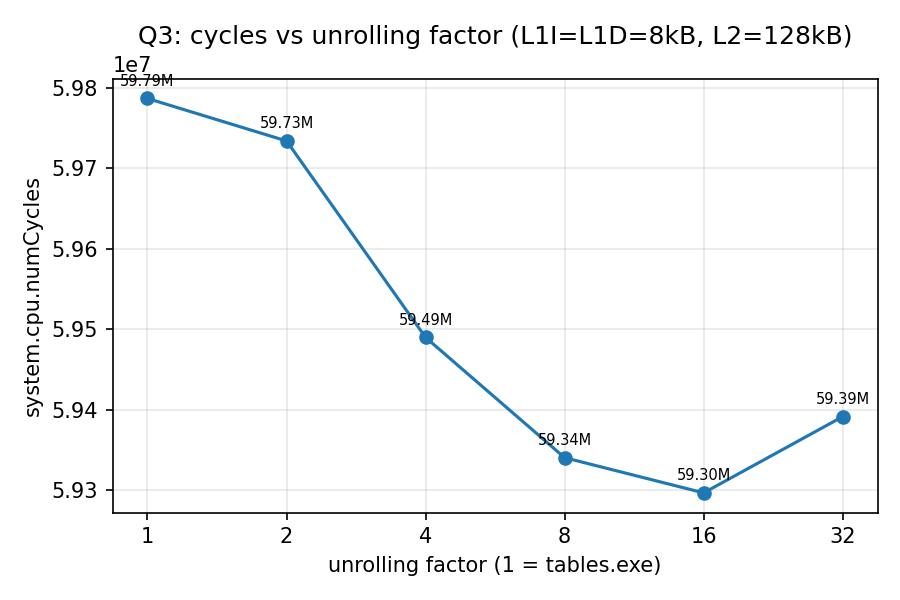
\includegraphics[width=0.68\linewidth]{../part2/results/q3_unrolling.png}
\caption{Κύκλοι εκτέλεσης συναρτήσει του unrolling factor.}
\label{fig:uf}
\end{figure}

Το unrolling μειώνει τους κύκλους, αλλά μόνο κατά 0,8\% στην καλύτερη περίπτωση (UF = 16).
Το όφελός του προέρχεται από το overhead του βρόχου: με \texttt{-O0} ο μετρητής \texttt{i}
βρίσκεται στο stack και σε κάθε επανάληψη γίνεται load, αύξηση, store και σύγκριση. Με UF = 16
οι προσβάσεις στην L1D πέφτουν από 4,44 σε 4,06 εκατομμύρια. Ο χρόνος όμως καθορίζεται από τα
L1D misses (περίπου 817 χιλιάδες), τα οποία το unrolling δεν επηρεάζει. Για UF = 32 οι κύκλοι
αυξάνονται ξανά. Ο κώδικας μεγαλώνει (7,3 KB στο \texttt{tables\_uf32.exe} έναντι 1,9 KB στο
\texttt{tables.exe}) και επιβαρύνει την L1I, χωρίς να μένει overhead βρόχου για να εξοικονομηθεί.
Η επίδραση αυτή φαίνεται πολύ πιο έντονα με μικρότερη L1I στο ερώτημα 4.

\textbf{Μέγεθος L1D.} Με \texttt{tables.exe}, L1I = 8~KB και L2 = 128~KB:

\begin{table}[H]
\centering
\caption{Κύκλοι εκτέλεσης και στατιστικά της L1D ανά μέγεθος L1D.}
\label{tab:l1d}
\begin{tabular}{@{}lcccccc@{}}
\toprule
L1D & 2 KB & 4 KB & 8 KB & 16 KB & 32 KB & 64 KB \\
\midrule
Κύκλοι (εκατ.) & 59,97 & 59,82 & 59,79 & \textbf{42,81} & 42,58 & 42,84 \\
L1D misses     & 824\,278 & -- & 816\,756 & 110\,454 & -- & 101\,993 \\
L1D miss rate  & 18,6\% & -- & 18,4\% & 2,5\% & -- & 2,3\% \\
\bottomrule
\end{tabular}
\end{table}

\begin{figure}[H]
\centering
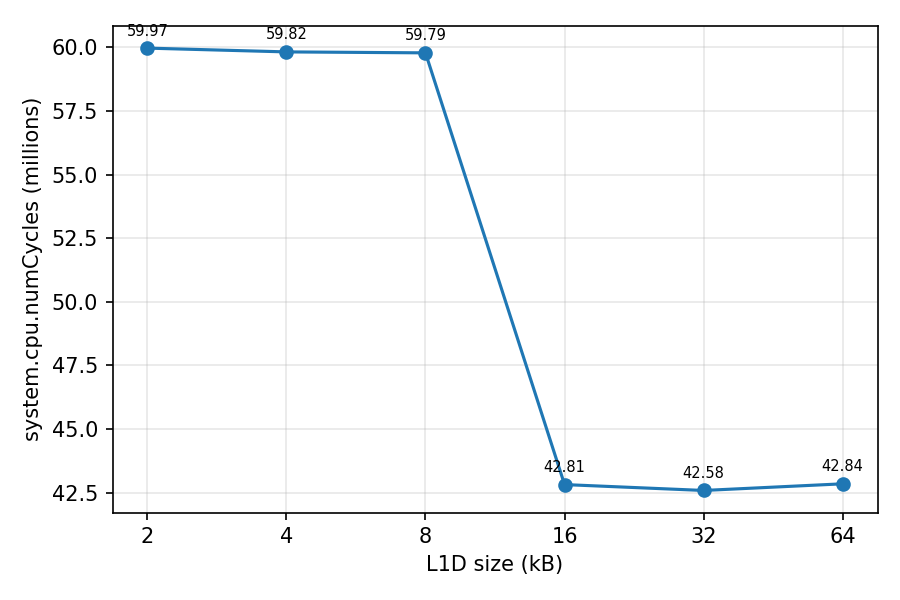
\includegraphics[width=0.68\linewidth]{../part2/results/q3_l1d.png}
\caption{Κύκλοι εκτέλεσης συναρτήσει του μεγέθους της L1D.}
\label{fig:l1d}
\end{figure}

Η καμπύλη δεν μειώνεται σταδιακά. Μένει σχεδόν σταθερή έως τα 8~KB, πέφτει απότομα κατά 28\%
στα 16~KB και μετά σταθεροποιείται ξανά. Η εξήγηση δεν είναι η χωρητικότητα: τα δεδομένα είναι
3,2~MB, πολύ περισσότερα από οποιαδήποτε από αυτές τις caches. Πρόκειται για \textbf{conflict
misses}.

Σε syscall emulation mode το gem5 δίνει φυσικές σελίδες τη στιγμή της πρώτης πρόσβασης. Ο βρόχος
αρχικοποίησης αγγίζει εναλλάξ τα \texttt{x1[i]}, \texttt{x2[i]}, \texttt{x3[i]} και
\texttt{y[i]}, οπότε οι σελίδες των τεσσάρων πινάκων καταλήγουν διαδοχικές στη φυσική μνήμη,
σε απόσταση 4~KB η μία από την άλλη. Οι εικονικές διευθύνσεις, που μετρήθηκαν μέσα στο gem5,
απέχουν 0xC4000 και έχουν όλες offset 0x010 μέσα στη σελίδα. Σε μια 2-way cache μεγέθους $C$
κάθε way καλύπτει $C/2$ bytes, και διευθύνσεις που διαφέρουν κατά πολλαπλάσιο του $C/2$
πέφτουν στο ίδιο set.

Για L1D $\le 8$~KB το way είναι το πολύ 4~KB, άρα και οι τέσσερις πίνακες αντιστοιχίζονται
στο ίδιο set. Κάθε επανάληψη χρειάζεται 4 γραμμές σε ένα set με 2 θέσεις, και κάθε πρόσβαση
διώχνει μια γραμμή που θα χρειαστεί αμέσως μετά (thrashing). Το αποτέλεσμα είναι περίπου ένα
miss ανά πρόσβαση σε πίνακα. Για L1D = 16~KB το way είναι 8~KB: τα \texttt{x1}, \texttt{x3}
μοιράζονται ένα set και τα \texttt{x2}, \texttt{y} ένα άλλο, οπότε οι δύο γραμμές κάθε set
χωράνε. Τα misses πέφτουν στις 110 χιλιάδες περίπου, πολύ κοντά στο ελάχιστο των compulsory
misses (3,2~MB / 64~B = 50\,000 γραμμές, μία φορά σε κάθε έναν από τους δύο βρόχους). Πάνω από
τα 16~KB δεν υπάρχει περαιτέρω κέρδος, αφού δεν υπάρχει επαναχρησιμοποίηση πέρα από τη γραμμή.

Για αυτό το μοτίβο προσβάσεων λοιπόν η associativity και η στοίχιση των δεδομένων μετρούν
περισσότερο από το καθαρό μέγεθος της cache. Συνέπεια του ίδιου φαινομένου είναι ότι για
L1D $\ge 16$~KB το L2 miss rate εκτοξεύεται (91,7\% για 16~KB): στην L2 φτάνουν πια μόνο τα
compulsory misses, τα οποία δεν μπορεί να εξυπηρετήσει.

\subsection*{4. Εξαντλητική αναζήτηση και Pareto front}

Ο χώρος σχεδίασης αποτελείται από L1I, L1D $\in \{2,\dots,64\}$~KB, L2 $\in \{128,\dots,1024\}$~KB
και unrolling factor $\in \{2,4,8,16,32\}$, δηλαδή $6 \cdot 6 \cdot 4 \cdot 5 = 720$ σημεία.
Όλες οι προσομοιώσεις εκτελέστηκαν με script. Κάθε προσομοίωση γράφει σε δικό της output
directory, ώστε να τρέχουν 10 παράλληλα, και το αποτέλεσμα αποθηκεύεται σε CSV.

\textbf{Χρόνος αναζήτησης.} Οι 720 προσομοιώσεις ολοκληρώθηκαν σε 688~s με 10 παράλληλες
εκτελέσεις. Το άθροισμα των επιμέρους χρόνων, δηλαδή ο χρόνος μιας σειριακής εξαντλητικής
αναζήτησης, είναι \textbf{114 λεπτά}.

Η καλύτερη καθυστέρηση είναι 41\,922\,998 κύκλοι (16/64/512~KB, UF = 16, 592~KB συνολικά)
και η χειρότερη 66\,060\,573 (2/2/128~KB, UF = 32). Το Pareto front υπολογίστηκε με τη
βιβλιοθήκη \texttt{paretoset} πάνω σε pandas dataframe με στήλες \texttt{totalMemoryKB}
(L1I + L1D + L2) και \texttt{latencyCC}, ελαχιστοποιώντας και τα δύο. Αποτελείται από
20 σημεία (Πίνακας~\ref{tab:pareto}, Σχήμα~\ref{fig:pareto}).

\begin{table}[H]
\centering
\small
\caption{Pareto-optimal αρχιτεκτονικές της εξαντλητικής αναζήτησης.}
\label{tab:pareto}
\begin{tabular}{@{}ccccrr@{}}
\toprule
L1I & L1D & L2 & UF & Μνήμη (KB) & Κύκλοι \\
\midrule
2 KB & 2 KB & 128 KB & 8 & 132 & 59\,581\,198 \\
2 KB & 4 KB & 128 KB & 8 & 134 & 59\,433\,698 \\
4 KB & 4 KB & 128 KB & 16 & 136 & 59\,343\,511 \\
4 KB & 8 KB & 128 KB & 16 & 140 & 59\,306\,017 \\
8 KB & 8 KB & 128 KB & 16 & 144 & 59\,296\,471 \\
\rowcolor{black!6} 2 KB & 16 KB & 128 KB & 8 & 146 & 42\,416\,612 \\
4 KB & 16 KB & 128 KB & 16 & 148 & 42\,409\,832 \\
8 KB & 16 KB & 128 KB & 16 & 152 & 42\,403\,308 \\
16 KB & 16 KB & 128 KB & 16 & 160 & 42\,387\,518 \\
2 KB & 32 KB & 128 KB & 8 & 162 & 42\,078\,234 \\
4 KB & 32 KB & 128 KB & 16 & 164 & 41\,969\,420 \\
8 KB & 32 KB & 128 KB & 16 & 168 & 41\,969\,226 \\
16 KB & 32 KB & 128 KB & 16 & 176 & 41\,945\,801 \\
32 KB & 32 KB & 128 KB & 16 & 192 & 41\,936\,488 \\
16 KB & 32 KB & 256 KB & 16 & 304 & 41\,933\,039 \\
64 KB & 32 KB & 256 KB & 16 & 352 & 41\,928\,359 \\
64 KB & 64 KB & 256 KB & 16 & 384 & 41\,925\,024 \\
16 KB & 32 KB & 512 KB & 16 & 560 & 41\,923\,846 \\
32 KB & 32 KB & 512 KB & 16 & 576 & 41\,923\,699 \\
16 KB & 64 KB & 512 KB & 16 & 592 & 41\,922\,998 \\
\bottomrule
\end{tabular}
\end{table}

\begin{figure}[H]
\centering
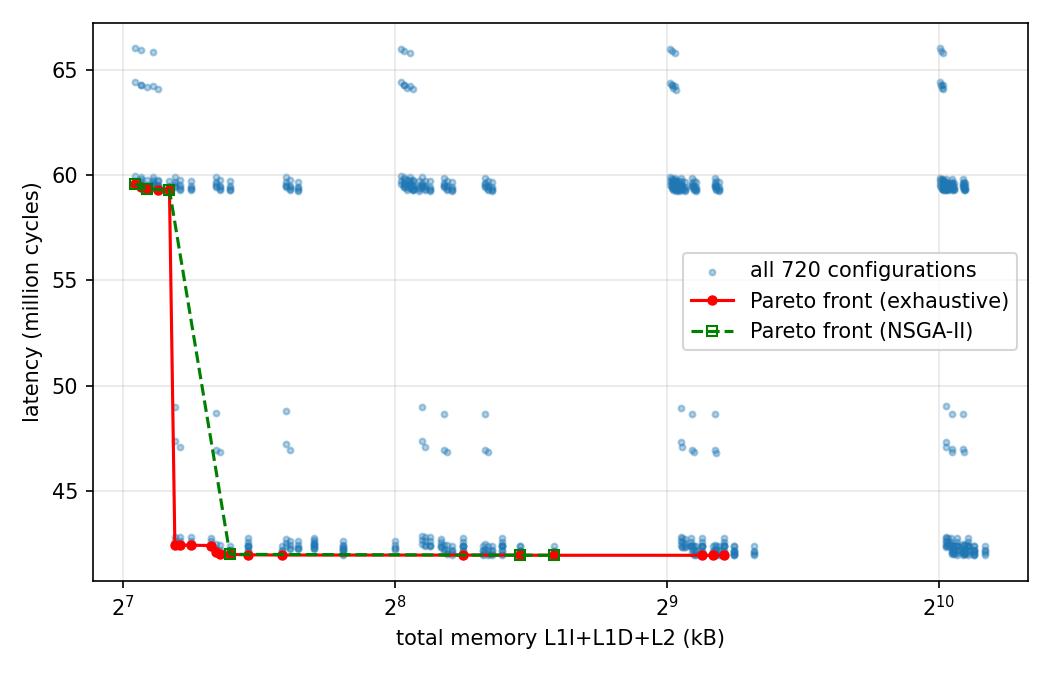
\includegraphics[width=0.78\linewidth]{../part2/results/q4_q5_pareto.png}
\caption{Οι 720 αρχιτεκτονικές, το Pareto front της εξαντλητικής αναζήτησης (κόκκινο) και
το Pareto front του γενετικού αλγορίθμου (πράσινο).}
\label{fig:pareto}
\end{figure}

Η παράμετρος που καθορίζει την απόδοση είναι η L1D. Η μετάβαση σε L1D $\ge 16$~KB, δηλαδή
η αποφυγή των conflict misses του ερωτήματος 3, μειώνει την καθυστέρηση κατά 29\% περίπου
με κόστος μόλις 2--14~KB μνήμης. Το «γόνατο» του front είναι η αρχιτεκτονική
\textbf{L1I 2~KB / L1D 16~KB / L2 128~KB με UF = 8} (146~KB, 42,4 εκατ. κύκλοι). Από εκεί και
πέρα κάθε επιπλέον μνήμη κερδίζει λιγότερο από 1,2\%.

Η L2 αντίθετα σχεδόν δεν επηρεάζει: η καλύτερη καθυστέρηση για κάθε μέγεθος L2 διαφέρει
λιγότερο από 0,05\%. Τα δεδομένα διαβάζονται μία φορά, οπότε μια μεγαλύτερη L2 δεν έχει τι να
επαναχρησιμοποιήσει, και γι' αυτό τα περισσότερα Pareto σημεία έχουν τη μικρότερη L2.

Τέλος, το unrolling αλληλεπιδρά με το μέγεθος της L1I, γιατί ένας βρόχος με μεγάλο unrolling
δεν χωράει σε μικρή L1I (Πίνακας~\ref{tab:l1iuf}). Με L1I 2~KB το καλύτερο UF είναι το 8, ενώ
με L1I $\ge 4$~KB είναι το 16. Αυτό εξηγεί γιατί τα Pareto σημεία μικρής μνήμης έχουν UF = 8.

\begin{table}[H]
\centering
\caption{Κύκλοι (εκατ.) ανά L1I και unrolling factor, για L1D = 32 KB και L2 = 128 KB.}
\label{tab:l1iuf}
\begin{tabular}{@{}lccccc@{}}
\toprule
L1I \textbackslash{} UF & 2 & 4 & 8 & 16 & 32 \\
\midrule
2 KB      & 42,45 & 42,24 & \textbf{42,08} & 46,95 & 48,68 \\
4 KB      & 42,40 & 42,19 & 42,03 & \textbf{41,97} & 46,85 \\
$\ge$ 8 KB & 42,39 & 42,18 & 42,01 & \textbf{41,97} & 42,16 \\
\bottomrule
\end{tabular}
\end{table}

\subsection*{5. Γενετικός αλγόριθμος}

Το \texttt{genOptimizer.py} του μαθήματος εκτελέστηκε χωρίς αλλαγές. Χρησιμοποιεί τον
NSGA-II της βιβλιοθήκης \texttt{pymoo} με πληθυσμό 10 και 5 απογόνους ανά γενιά, και το
κριτήριο που τον σταματά εδώ είναι το μέγιστο των 5 γενεών. Έκανε \textbf{30 evaluations}
($10 + 4 \times 5$) σε \textbf{215~s}. Αυτό αντιστοιχεί στο 4,2\% των προσομοιώσεων της
εξαντλητικής αναζήτησης και σε περίπου 32 φορές μικρότερο χρόνο από τη σειριακή εκδοχή της
(114 λεπτά). Το Pareto front που επέστρεψε φαίνεται στον Πίνακα~\ref{tab:ga}.

\begin{table}[H]
\centering
\caption{Pareto front του γενετικού αλγορίθμου και σύγκριση με το πραγματικό.}
\label{tab:ga}
\begin{tabular}{@{}ccccrrl@{}}
\toprule
L1I & L1D & L2 & UF & Μνήμη (KB) & Κύκλοι & Στο πραγματικό front; \\
\midrule
2 KB  & 2 KB  & 128 KB & 8  & 132 & 59\,581\,198 & ναι \\
4 KB  & 4 KB  & 128 KB & 16 & 136 & 59\,343\,511 & ναι \\
8 KB  & 8 KB  & 128 KB & 16 & 144 & 59\,296\,471 & ναι \\
8 KB  & 32 KB & 128 KB & 16 & 168 & 41\,969\,226 & ναι \\
32 KB & 64 KB & 256 KB & 16 & 352 & 41\,929\,862 & όχι \\
64 KB & 64 KB & 256 KB & 16 & 384 & 41\,925\,024 & ναι \\
\bottomrule
\end{tabular}
\end{table}

Τα 5 από τα 6 σημεία είναι πράγματι Pareto-optimal. Το έκτο (32/64/256~KB) κυριαρχείται
οριακά από την αρχιτεκτονική 64/32/256~KB, που έχει την ίδια συνολική μνήμη και 1\,503 κύκλους
λιγότερους. Ο αλγόριθμος βρήκε όμως μόνο 5 από τα 20 σημεία του πραγματικού front και, κυρίως,
\textbf{έχασε το γόνατο}: κανένα σημείο του δεν έχει L1D = 16~KB. Έτσι, μεταξύ 144 και 168~KB
το front του δίνει ακόμη 59 εκατ. κύκλους, ενώ με 146~KB επιτυγχάνονται ήδη 42,4 εκατ.
(Σχήμα~\ref{fig:pareto}).

Ο γενετικός αλγόριθμος δίνει τη γενική μορφή του trade-off (μικρή και αργή αρχιτεκτονική
απέναντι σε μεγάλη και γρήγορη) με ένα κλάσμα του κόστους, αλλά με 5 γενεές και πληθυσμό 10
δεν προλαβαίνει να συγκλίνει. Περισσότερες γενεές ή μεγαλύτερος πληθυσμός θα έκλειναν τη
διαφορά με περισσότερες προσομοιώσεις. Εδώ η εξαντλητική αναζήτηση ήταν εφικτή μόνο επειδή
κάθε προσομοίωση διαρκεί περίπου 9~s. Σε μεγαλύτερο χώρο σχεδίασης, ή με πιο αργές
προσομοιώσεις, η ευρετική αναζήτηση είναι η μόνη ρεαλιστική επιλογή.

% ============================== ΠΑΡΑΡΤΗΜΑ ==============================
\section*{Παράρτημα: Κώδικας}
\addcontentsline{toc}{section}{Παράρτημα}

Όλος ο κώδικας και τα δεδομένα των μετρήσεων βρίσκονται στο\\
\url{https://github.com/Zajason/embedded_systems/tree/main/lab/Lab1}.

\begin{itemize}
\item \texttt{src/}: ο κώδικας της πλακέτας. Το \texttt{hal\_entry.c} χρονομετρά όλες τις
      εκδόσεις. Ο αρχικός αλγόριθμος βρίσκεται στο \texttt{phods\_baseline.h} και το v1 στο
      \texttt{phods\_variants.h}. Από τον βελτιστοποιημένο κώδικα του \texttt{phods\_impl.h}
      παράγονται τα v2--v4 και οι 16 εκδόσεις $B_x \times B_y$.
\item \texttt{test/host\_test.c}: έλεγχος ορθότητας όλων των εκδόσεων σε υπολογιστή.
\item \texttt{tools/analyze.py}: μετατροπή των μετρήσεων της πλακέτας σε CSV και διαγράμματα.
\item \texttt{part2/scripts/}: τα scripts του gem5 (ερωτήματα 1--5) και
      \texttt{part2/results/}: όλα τα αποτελέσματα σε CSV.
\end{itemize}

\end{document}
